

\documentclass{acm_proc_article-sp}
\usepackage{multicol}
\usepackage{nicefrac}
\begin{document}

\title{Cluster Based Content Distribution in VANETs}


\numberofauthors{2} 
\author {
% 1st. author
\alignauthor
Aravindan Balan\\
       \email{aravindan@cs.ucla.edu} 
\\
University of California Los Angeles\\
       \and    
% 3rd. author
\alignauthor 
Mario Gerla\\
       \email{gerla@cs.ucla.edu}
\\
University of California Los Angeles\\
}


\maketitle
\begin{abstract}
\vspace{1 mm}
The communication-enabled vehicles are interested in downloading different multimedia contents
from Internet-based servers. This system captures many of the entertainment services with
effective information, such as navigation maps, news reporting service, and software updating, or multimedia content downloading. In this approach both infrastructure-to-vehicle and vehicle-vehicle communication take place. It also demands for better performance due to existing difficulties and challenges including limited RSUs available on the road, expensive and limited 3G/LTE resource, etc. By introducing the idea of peer-to-peer content delivery to vehicular networks, cooperative schemes, such as SPAWN \cite{spawn}, significantly improve the efficiency of content downloading in vehicular networks, where the cooperation among vehicles is essential to establish such systems. Hence, uncooperative behavior of peers can severely degrade the system performance, e.g. some vehicles may avoid downloading original data chunks through 3G network in order to save the cost of 3G connection, and only wait for other peers to share with him, i.e. choose to be a free-rider. On the other hand, if too many nodes connect to the 3G/LTE, the 3G/LTE network may encounter serious congestion, and it would be a waste of network resource if many of them are actually downloading the same content.

In this paper, we have proposed a cluster based content distribution scheme for Vehicular Adhoc Networks. Vehicles with common interests form a cluster and take turns to be the cluster head that directly downloads data packets in multiple rounds, especially multimedia content, from the Internet and share with others in the cluster. Our work is mainly focused on highway scenarios in VANETs as vehicles tend to stick together for a considerable amount of time. We have also proposed a novel technique for cluster head selection and also consider other scenarios where vehicles are selfish. We have also investigated the optimal parameters to use to obtain a proper trade-off between efficiency/congestion of the LTE network versus the Robustness of the system. Finally, we have analysed the results on how the selection of optimal parameters affects the network condition. The functionality of our proposed network is verified using ns-3 and SUMO simulations. 

\end{abstract}

\keywords{Peer-to-Peer, Vehicular ad-hoc Network, Multimedia Content Downloading, Cooperative Content Downloading, Cluster-based Content Downloading}

\begin{figure}
\centering
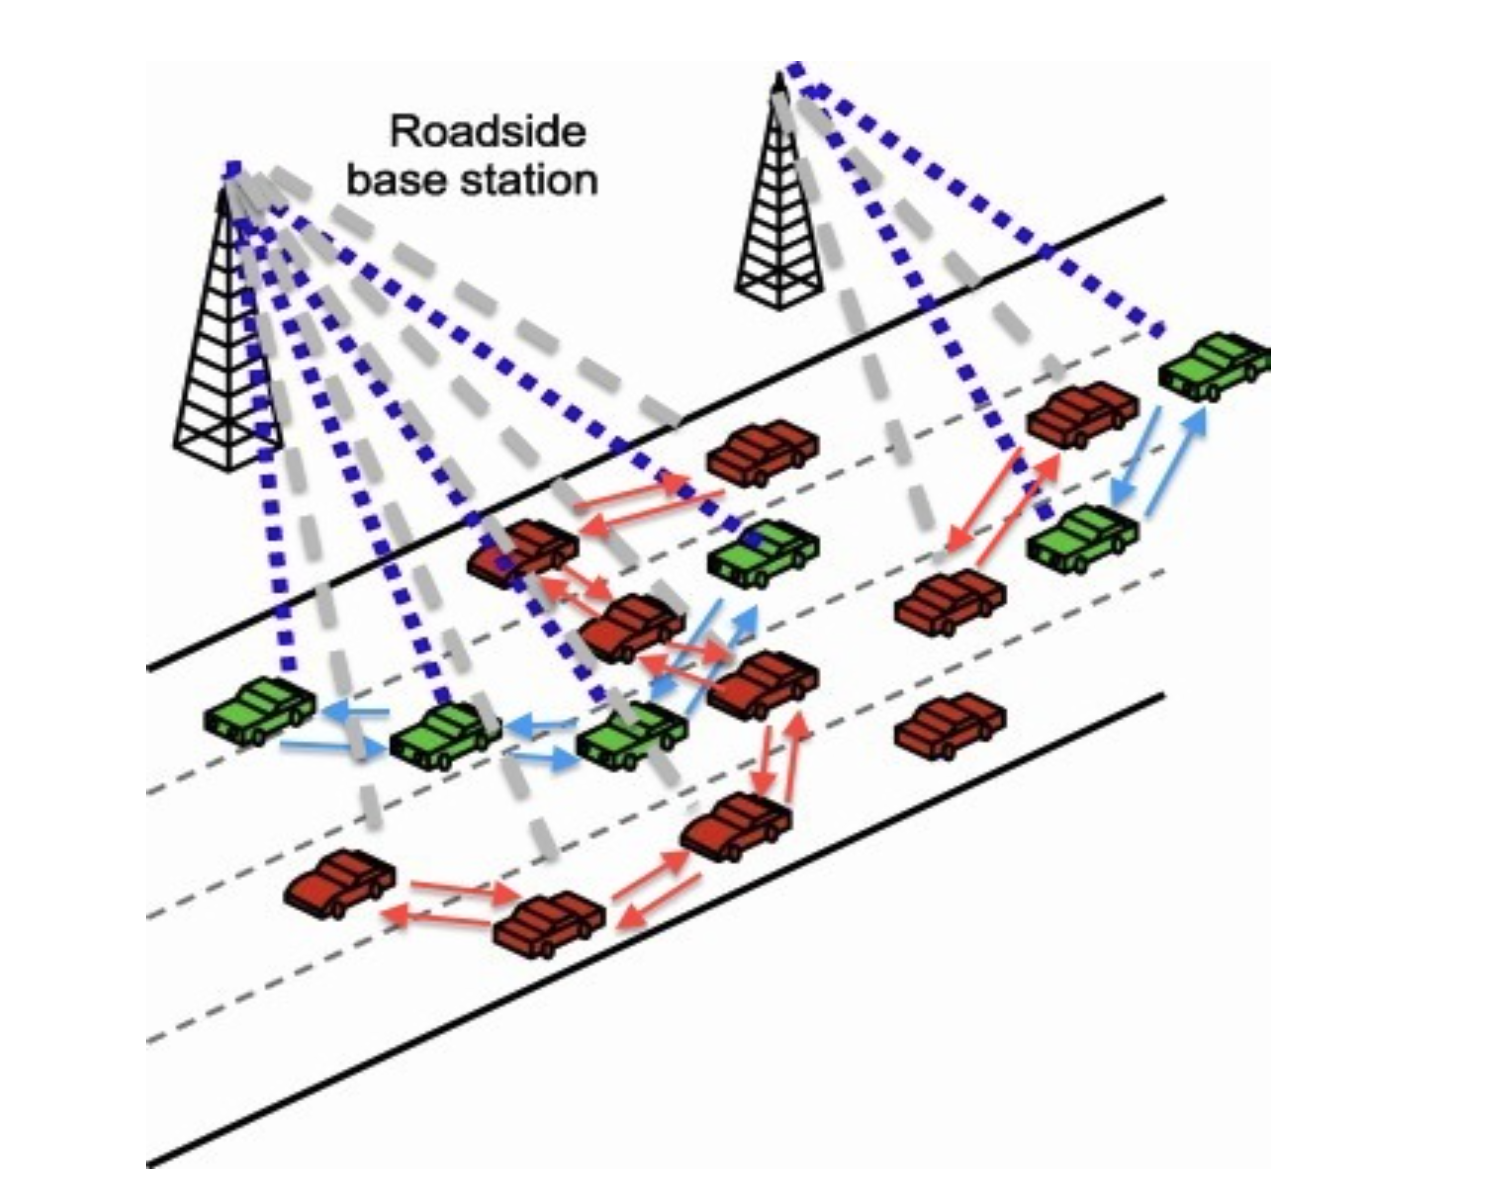
\includegraphics[scale=.33]{working.png} \caption{Cluster Based Content Distribution in VANETs}
\label{working}
\end{figure}

\section{Introduction}
\vspace{1 mm}

Vehicular Ad-hoc Network (VANET) is one of the most emerging areas for the improvement of Intelligent Transportation System (ITS). VANET is a special form of MANET, where Mobile Ad-hoc Network (MANETs) are self-configuring network of mobile nodes connected by wireless links, while, VANET are distributed and self-assembling communication networks. A technology that uses moving vehicles as nodes to create a mobile network is termed as VANET. Here, node movement is restricted by factors like road course, encompassing traffic and traffic regulations. The
primary goal of VANET is to provide road safety and other value added services such as email, audio/video sharing etc.

In the near future, the proliferation of "smart vehicles" is envisaged to become a reality. "Smart vehicles" combine the advantages of both smartphones and laptops: they are as "mobile" as smart phones, i.e. having ubiquitous access to the Internet via 3G/LTE networks, but more powerful in computation and energy supply like laptop computers. Beside safety services, content downloading is expected to be widely popular among drivers and passengers aboard just
like traditional networks. Since the number of road side units is very limited, the time that vehicles can get access to WiFi is very short. So for most of the time, vehicles rely on 3G/LTE to download the contents. However, as data files, such as pictures, audios and videos, are getting larger and larger due to the increasing demands of higher quality of user experience, the 3G/LTE resources, on the contrary, are getting more and more scarce and thus expensive. So the bandwidth assigned to each 3G user is limited which results in long delay of content downloading.

As inter-vehicle communication technology becomes available, cooperative content downloading schemes are proposed to leverage this advantage and bring peer-to-peer overlay network to the vehicular environment. As a typical example, SPAWN \cite{spawn} is a peer-peer content delivery mechanism that utilizes parallel download among a mesh of co-operating peers. Given a very limited amount of RSUs, most of the time, vehicles with common content interest download pieces/chunks of data from the Internet through cellular base stations and share with each other in adhoc mode, as shown in Figure \ref{working}. Such cooperative downloading scheme significantly improve the efficiency of content downloading and shorten the delay.

\section{Related Work}
\vspace{1 mm}

Most existing approaches that improve the efficiency of content downloading in vehicular networks, such as \cite{urban}, \cite{symbol}, \cite{cost}, \cite{opti}, \cite{ondemand}, \cite{datadissem}, rely on the cooperation among vehicles. However, misbehavior among the vehicle community motivated by selfish intentions of saving 3G/LTE bandwidth or energy can severely interfere the network performance. Hence incentive schemes are necessary to enforce the cooperation among nodes in vehicular networks. Incentive schemes, such as \cite{coalitional}, \cite{coop}, \cite{incentive}, \cite{uncoop}, are proposed to enforce the cooperation of intermediate nodes to forward packets in VANETs. Generally, incentive schemes can be categorized into two types, i.e. credit based schemes and reputation based schemes. Credit based schemes are adopted by \cite{coalitional}, \cite{incentive}, \cite{uncoop} where rewards/credits are allocated/paid to the forwarders. A three-counter scheme was proposed in \cite{coop} where nodes count the number of packets for- warded and the number of packets requested to be forwarded as a way of observing and recording the behavior of neighbor nodes, which is fairly similar to the way reputation schemes work. 

\begin{figure}
\centering
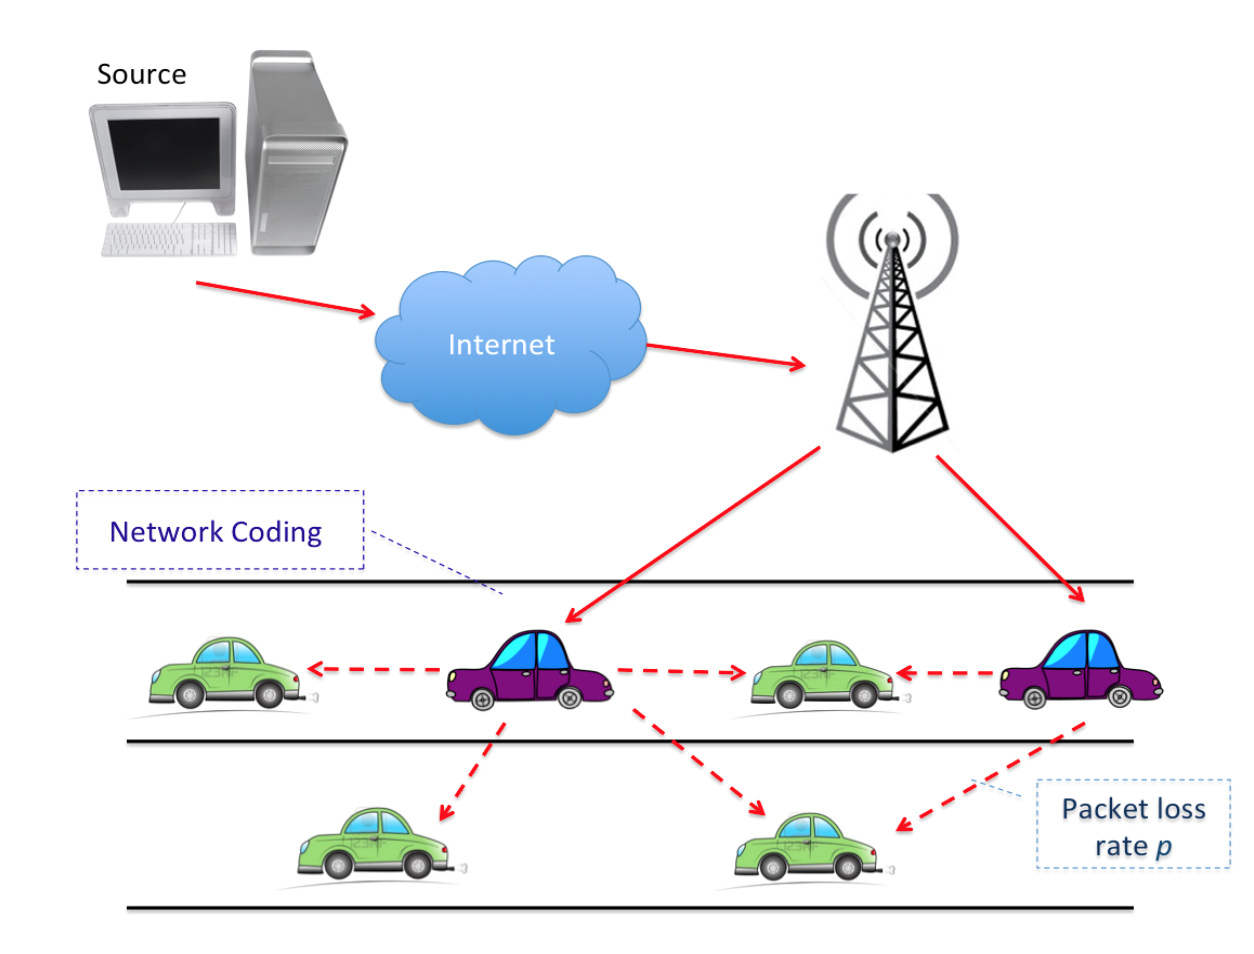
\includegraphics[scale=.30]{design.png} \caption{Overall Design of the System}
\label{design}
\end{figure}

As a matter of fact, the power supply for vehicles is not as a critical issue as for mobile devices, hence nodes in VANETs usually do not have strong intentions to drop the packets from other vehicles in order to save energy. However, 3G/LTE bandwidth is always a scarce resource, no matter for smart phones or smart vehicles. While some smart vehicles download interesting contents from the Internet via 3G/LTE and share with the neighborhood in V2V manner, selfish vehicles may have intentions to be free-riders who benefit from the contributing nodes but refuse to be the contributor itself in order to save its 3G/LTE bandwidth. As to our knowledge, so far there is no incentive scheme designed to enforce the cooperative downloading and maintain fairness for vehicular networks.

\section{ SYSTEM MODEL AND Design}
\vspace{1 mm}

\subsection{Network Model}
\vspace{1 mm}
We consider vehicular networks where vehicles with the same interested contents form a cluster, as shown in Figure \ref{design}. Our model is similar to \cite{game}, in which a few cluster heads are selected and they download the original data contents from the Internet source via 3G/LTE network. The cluster heads share their data packets with other vehicles in the cluster, and others may share with each other in a peer-to-peer fashion. Since the highly mobile vehicular network usually has a significant packet loss rate, in order to cope with the link loss, the cluster heads should perform network coding (with or without redundancy added) before broadcasting the data. A vehicle may receive network coded packets from different cluster heads, but still can decode and reconstruct the original content, similar to the way how a classical multi-path network coding scheme works.

The topic clusters in the system are managed by a Cluster Manager which acts as a remote server. The Cluster Manager is responsible for various functions like multi-round content delivery, topic cluster formation, cluster head selection, vehicle churning (vehicles entering and leaving the cluster). 

Our focus was mainly on the Highway scenario of VANET where we can expect lesser node churning and the clusters are intact for a considerable amount of time as compared to Urban scenarios. We have designed a server-assisting scheduling scheme that both enforces cooperation of vehicles, guarantees sufficiency of cluster head volunteers and efficiency of deciding who is next to be the cluster head. 

\subsection{System Design}
\vspace{1 mm}
Initially, vehicles express their interest in a particular topic to the Cluster Manager server application residing in the RSUs. The cluster manager tries to find a nearby cluster group of same topic of interest or forms a new cluster and add the vehicles either to the respective clusters. 

The Cluster manager server application fetches the topic content from the content source and encrypts the raw content, such as a video stream, with a temporary key. The key is updated periodically. The data packets are sent in multiple rounds to avoid fragmentation losses due to large packet sizes. The Cluster Manager broadcasts the topic packets to all the masters in the system chosen for that round. Only those masters interested in that particular topic receive the packet. 

The cluster heads then perform network coding (with or without redundancy added) and broadcasts the packet again to all other nodes in the cluster. A vehicle may receive network coded packets from different cluster heads, but still can decode and reconstruct the original content. Also the Cluster manager selects different masters for each round from each cluster thereby ensuring equal participation of all vehicles and avoid selfish vehicles. 
 
\subsection{Cluster Head Selection Algorithm}
\vspace{1 mm}
We have proposed an novel and an optimal cluster head selection algorithm. Choosing the right cluster head has a direct impact on the system performance. The cluster Manager chooses the optimal clusters heads for each round before broadcasting the packets to the masters which later distributes them to the edge nodes through network coding. So choosing a cluster head which is far away from the RSU might cause packet losses in the first stage. Also if a closer cluster head is chosen, it might cause packet losses while distributing it to the edge nodes as it might be far away. Since vehicles are constantly moving on an highway,thus choosing the optimal cluster head significantly improves the system performance. 

Cluster head selection algorithm works as follows. Firstly, a list of possible cluster head candidates are chosen based on the distance (range threshold) from the RSUs. Then we choose random candidates from this candidate list to be the cluster heads for this round. As an enhancement over the key management scheme defined, we also maintain a cache of the previously chosen cluster heads which ensures that only nodes which have not been masters before are chosen and all nodes in the system get fair participation. This prevents the selfish nature of nodes. If there aren't enough candidates for cluster heads, we choose the remaining candidates randomly from the previous chosen master set and the cache is cleared to make all nodes in the system eligible for the next round. 

\subsection{Server-Assisting Key Management Scheme}
\vspace{1 mm}
We have proposed a server-assisting incentive based key management scheme. As mentioned earlier in the paper, all data packets are encrypted with a temporary key and the key is rotated periodically. The server rewards the cluster heads by giving them the keys for the next a few periods after they have been serving as cluster head for a certain amount of time. So for the next a few periods, those previous cluster heads will be able to decode the content. Those who have never been a cluster head before are not able to decode, even if they can receive the content by overhearing the V2V broadcast. Hence they have to volunteer to serve as a cluster head in order to receive the key from the server. This server-assisted key management scheme ensures fair participation of all vehicles.

Cluster head global cache along with the key management scheme ensures better vehicle participation thereby preventing uncooperative vehicles(Free riders) degrading the system performance. 

\begin{figure}
\centering
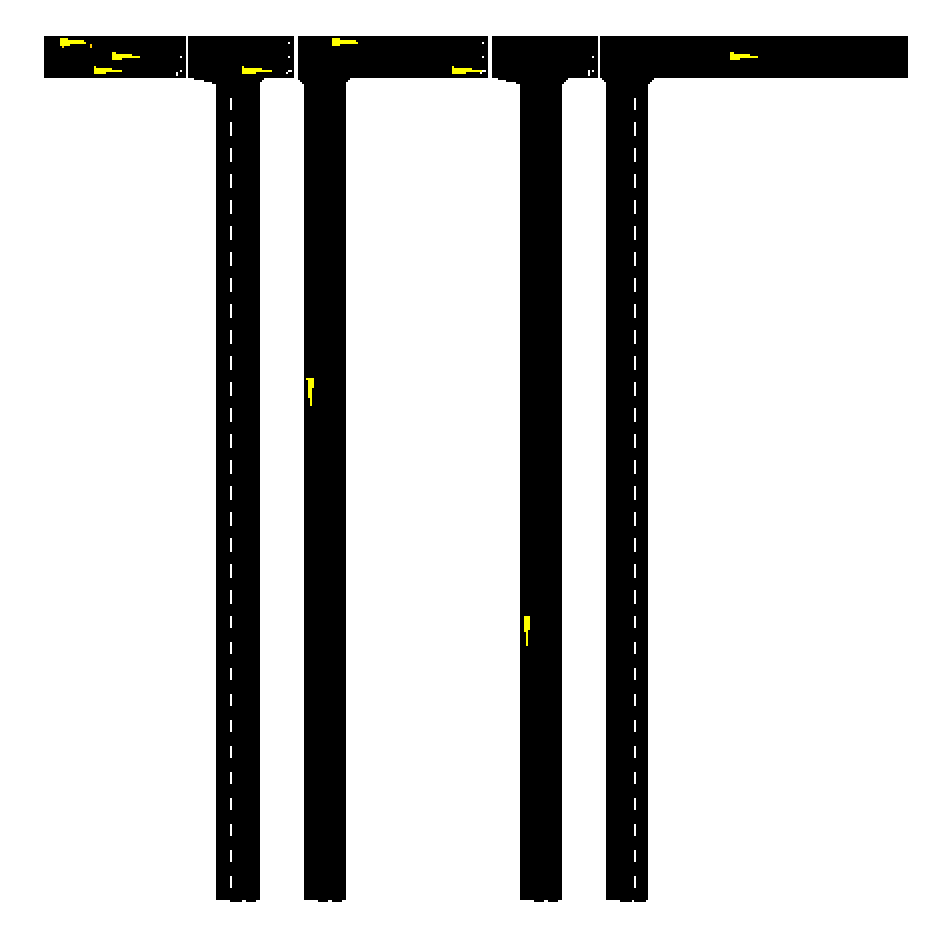
\includegraphics[scale=.40]{sumo.png} \caption{SUMO Highway Layout}
\label{sumo}
\end{figure}


\section{Vanet Simulation Details}
\vspace{1 mm}

We have simulated the Vanet Highway scenario using SUMO and NS3 \cite{sumons3}.   

\subsection{Simulation tools and platforms}
\vspace{1 mm}
\subsubsection{Simulation of Urban Mobility}
\vspace{1 mm}
Simulation of Urban Mobility (SUMO) \cite{sumo} is an open source traffic simulation package including net import and demand modelling components. SUMO helps to investigate several research topics e.g. route choice and traffic light algorithm or simulating vehicular communication.the framework is used in different projects to simulate automatic driving or traffic management strategies. Simulations has: space-continuous and time-discrete vehicle movement, different vehicle types, multi-lane streets with lane changing, different right-of-way rules, traffic lights, a fast open GL graphical user interface, manages networks with several edges, fast execution speed, interoperability with other application at run-time, network-wide, edge-based, vehicle-based, and detector-based outputs, supports person-based inter-modal trips, high portability and high interoperability.

\subsubsection{NS-3}
\vspace{1 mm}
NS-3  \cite{ns} is a discrete-event network simulator and a free software which succeeds popular network simulator NS-2.

We have simulated the system using Network Simulator-3 (NS-3). NS-3 is built using C++ and Python with scripting capability. NS-3 is well suited for wireless simulations which involve models for Wi-Fi, WiMAX, or LTE for layers 1 and 2 and routing protocols such as OLSR and AODV.

\subsection{Simulation parameter specifications}
\vspace{1 mm}
We have designed the highway layout  as shown in Figure \ref{sumo} with 50 vehicles moving at velocity of 60 mph, 1 stationary RSU, 3 lanes, 4 highway exits. We have mainly focused mainly on the vehicles exiting the system as SUMO is particularly designed for Urban scenarios where vehicles stop before a junction and not for Highway scenarios where vehicles don't stop while entering a highway. Also the Stationary RSU is placed in the middle of the highway for simulation purposes. 

We used the trace file generated using SUMO to define the mobility of all the nodes in NS-3. So the nodes created in ns3 correspond to the vehicles defined in SUMO. We have also induced a Range Propagation Loss Model with a range of 30 meters. 



\begin{figure}
\centering
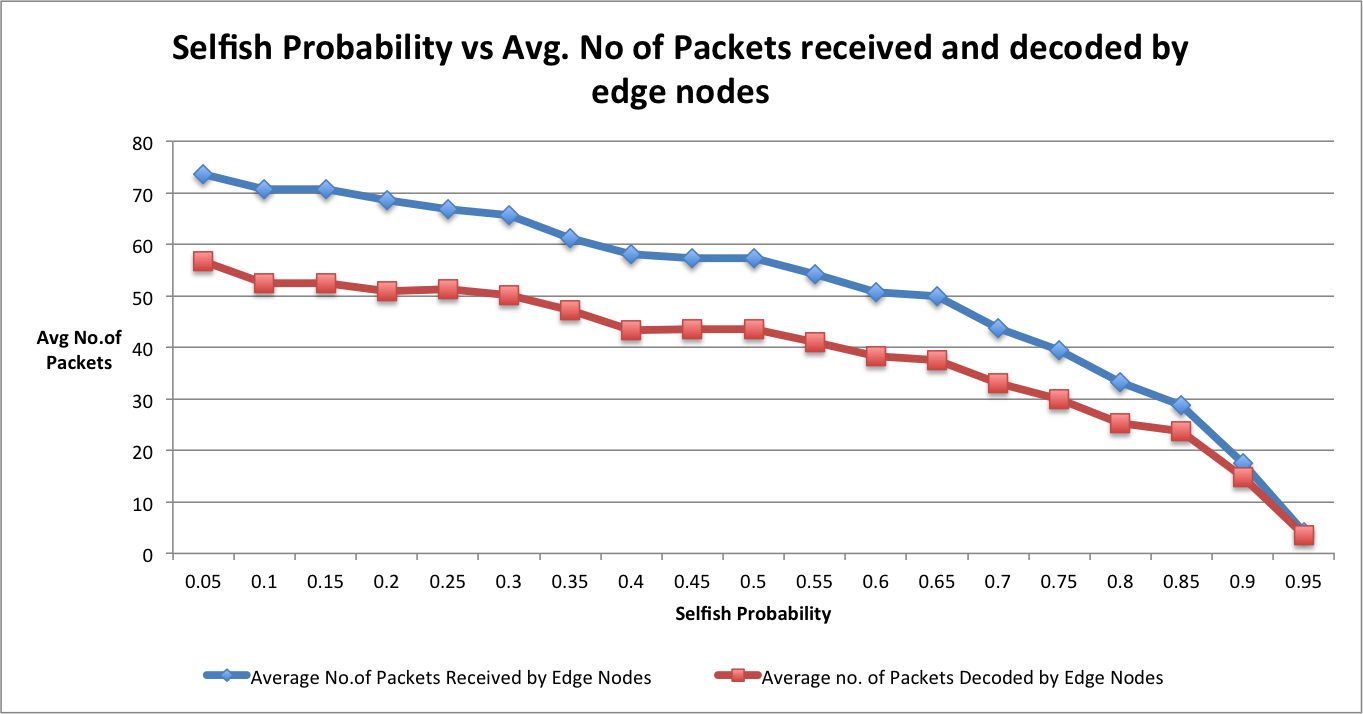
\includegraphics[scale=0.37]{selfprob.png}
\caption{Selfish Probability versus Average Number of Packets Received and Decoded by Edge Nodes}
\label{selfprob}
\end{figure}


\begin{figure*}[ht]
\begin{minipage}[b]{0.50\linewidth}
\centering
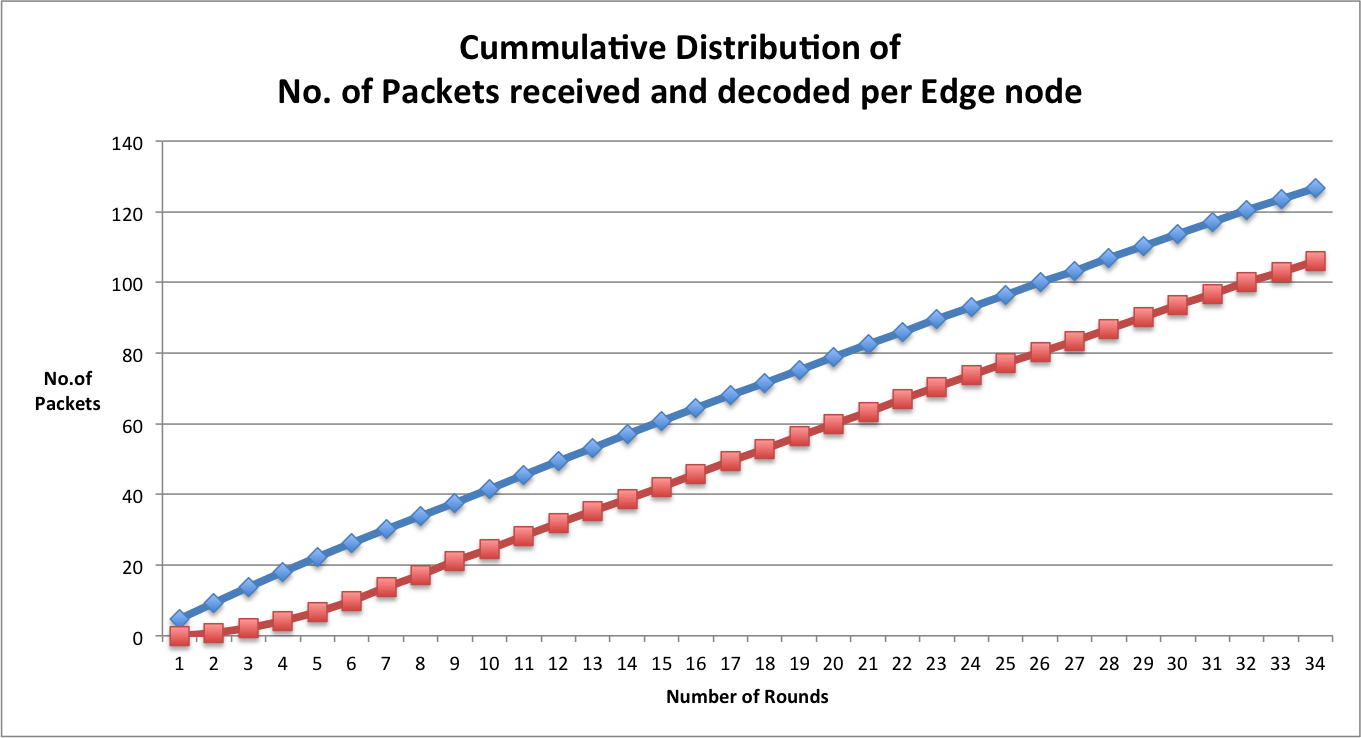
\includegraphics[width=\textwidth]{cummdistroundsvsavgpkt.png}
\caption{Cummulative Distribution of Number of Rounds versus Average Number of Packets Received and Decoded by Edge Nodes}
\label{cummdistroundsvsavgpkt}
\end{minipage}
\hspace{0.5cm}
\begin{minipage}[b]{0.50\linewidth}
\centering
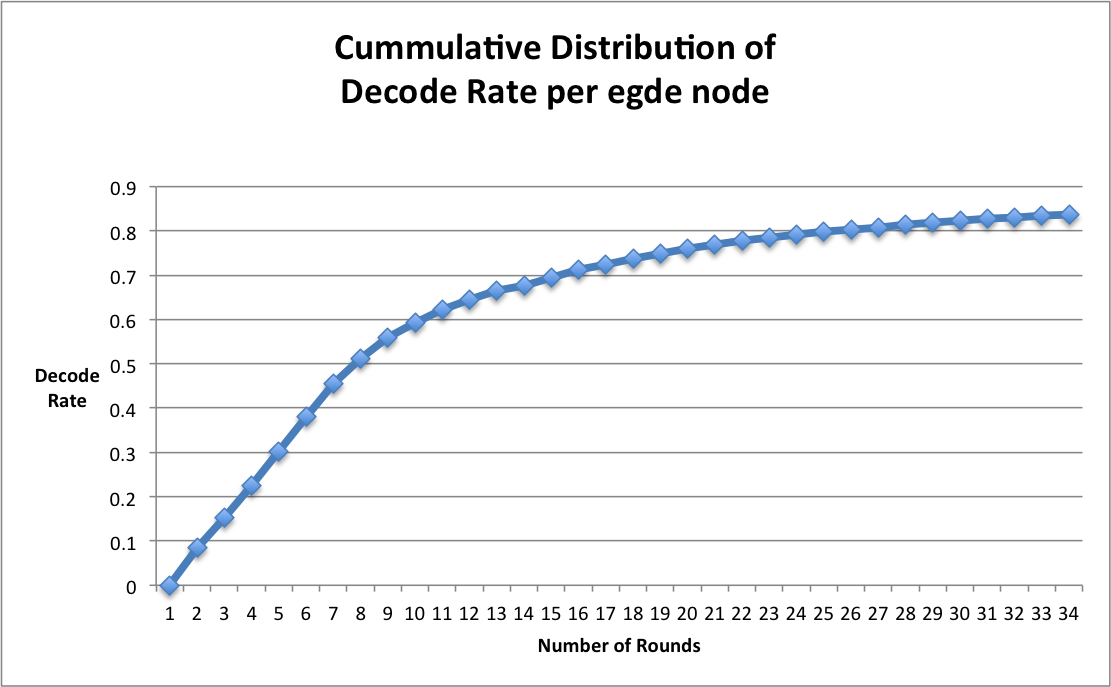
\includegraphics[width=\textwidth]{cummdistnumroundsvsdecoderate.png}
\caption{Cummulative Distribution of Number of Rounds versus Decode Rate}
\label{cummdistnumroundsvsdecoderate}
\end{minipage}
\end{figure*}

\begin{figure*}[ht]
\begin{minipage}[b]{0.50\linewidth}
\centering
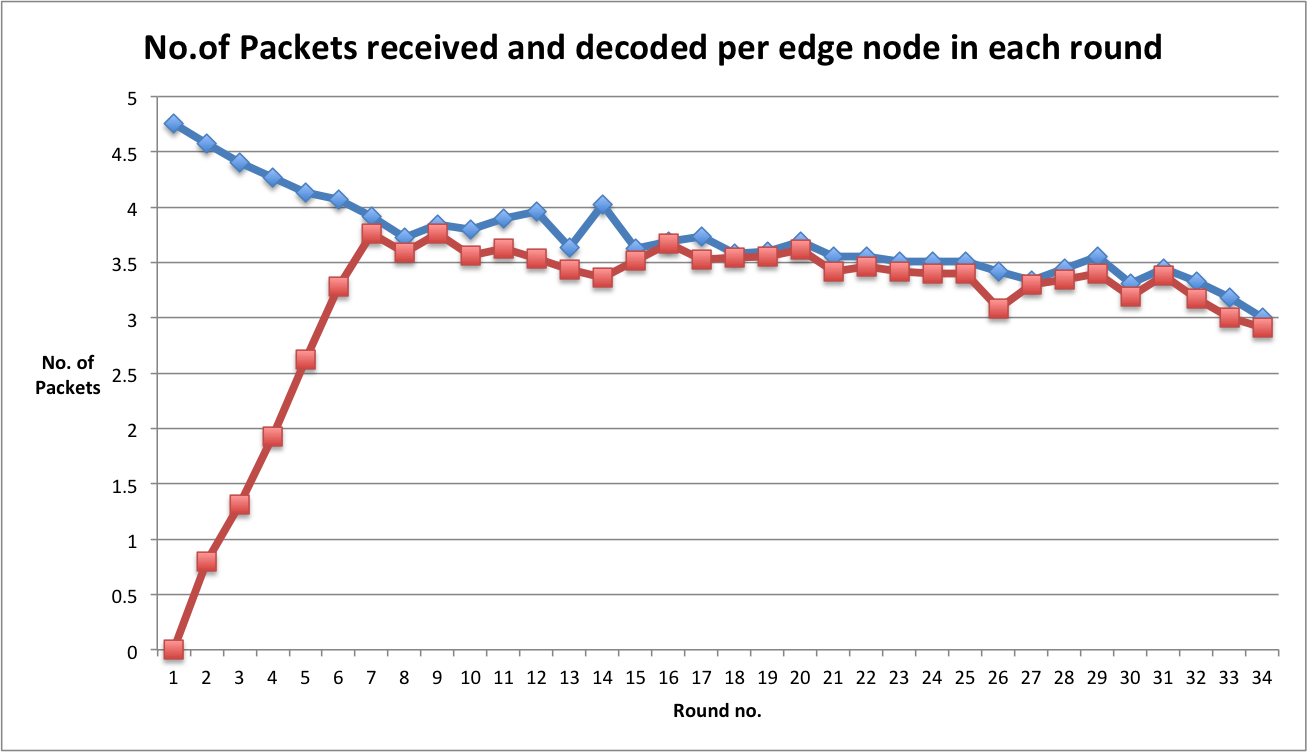
\includegraphics[width=\textwidth]{numpacketrecdecodeperroundperedge.png}
\caption{Average Number of Packets Received and Decoded by Edge Nodes per round}
\label{numpacketrecdecodeperroundperedge}
\end{minipage}
\hspace{0.5cm}
\begin{minipage}[b]{0.50\linewidth}
\centering
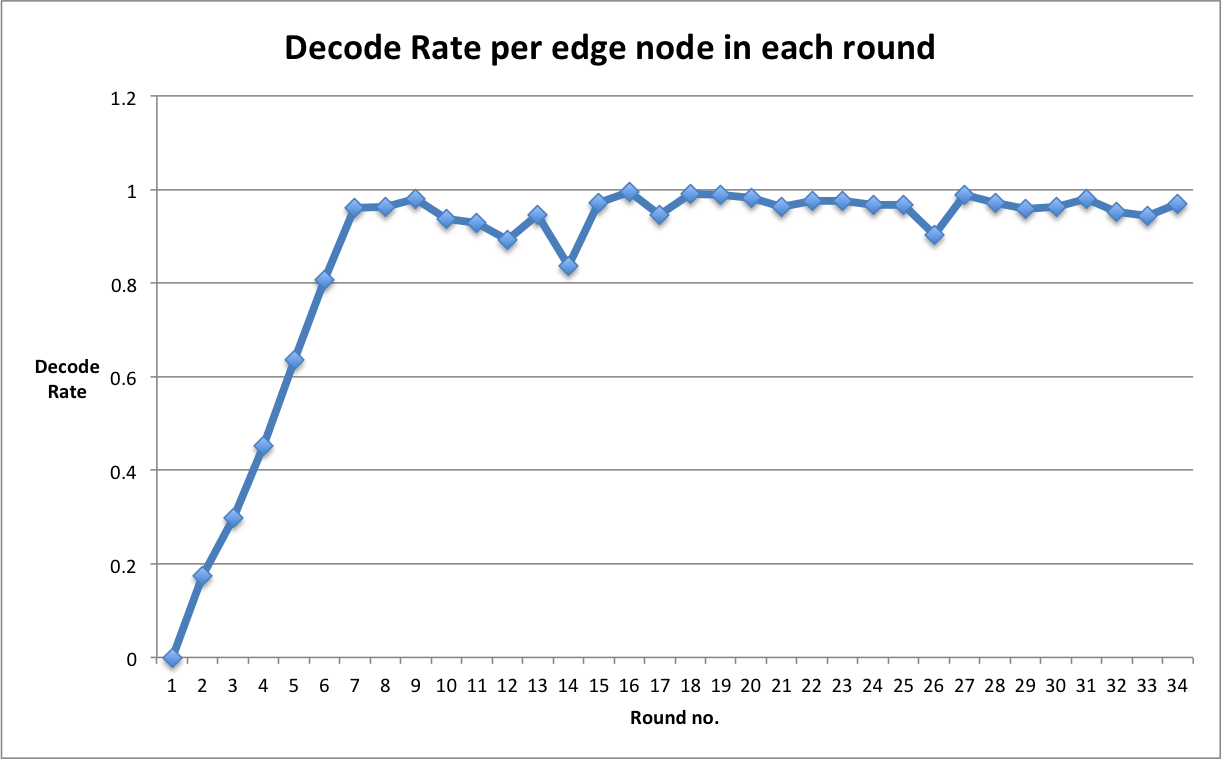
\includegraphics[width=\textwidth]{decoderateperroundperedge.png}
\caption{Decode Rate of Edge nodes per round}
\label{decoderateperroundperedge}
\end{minipage}
\end{figure*}

\begin{figure*}[ht]
\begin{minipage}[b]{0.50\linewidth}
\centering
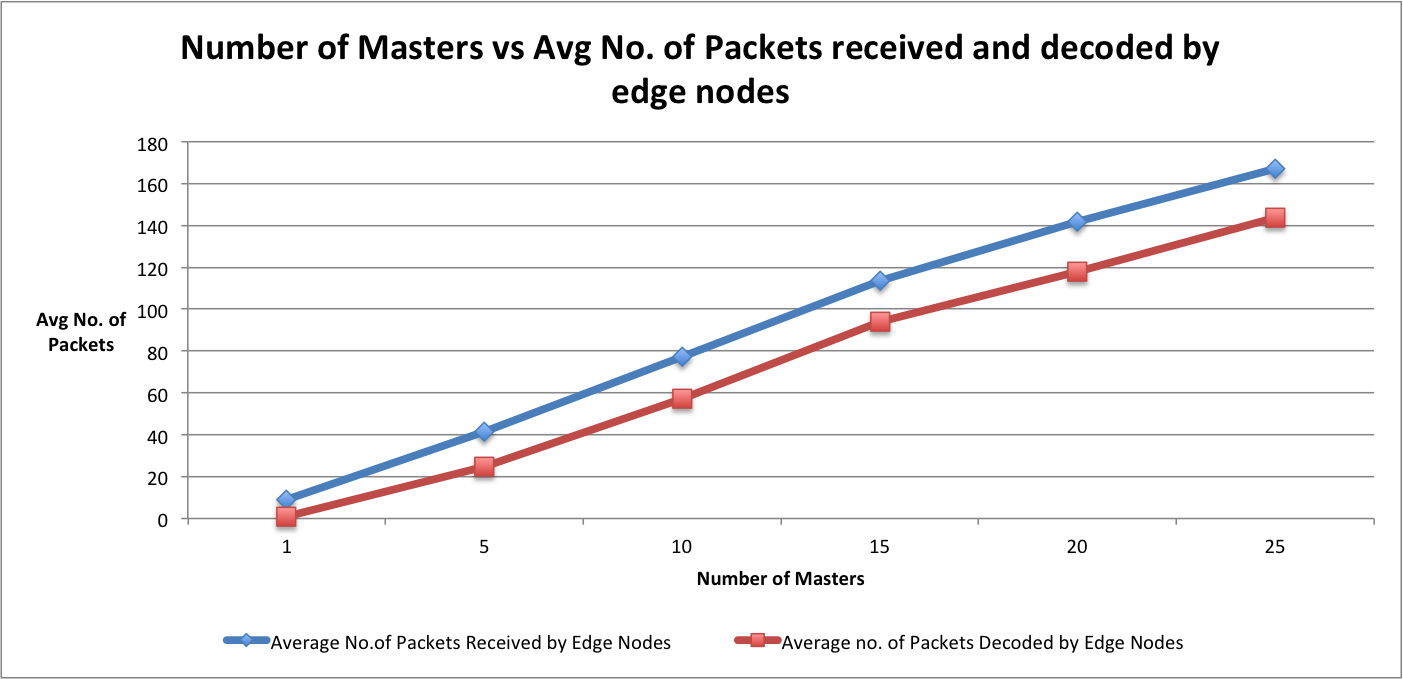
\includegraphics[width=\textwidth]{nummasters.png}
\caption{Number of Cluster Heads versus Average Number of Packets Received and Decoded by Edge Nodes}
\label{nummasters}
\end{minipage}
\hspace{0.5cm}
\begin{minipage}[b]{0.50\linewidth}
\centering
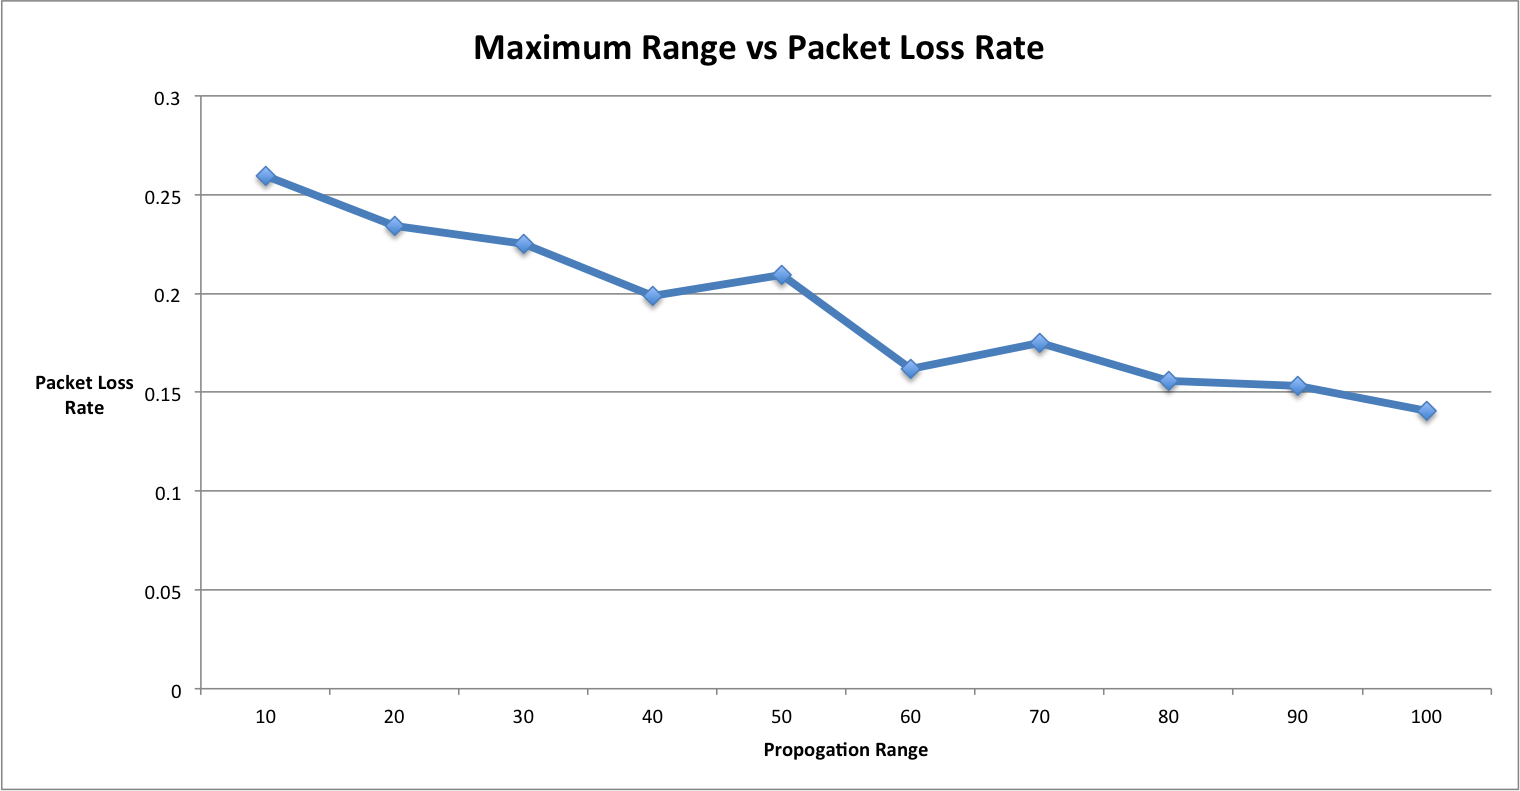
\includegraphics[width=\textwidth]{maxrange.png}
\caption{Maximum Propagation Range versus Packet Loss Rate}
\label{maxrange}
\end{minipage}
\end{figure*}




\section{Experimental Results}
\vspace{1 mm}

To quantify the performance of the system, experiments were done using the ns-3 network simulator with the help of SUMO. 

We have taken multiple scenarios and parameters into consideration. We have analysed the average number of packets received and decoded, decode rate, packet loss rate for each edge node by varying the following parameters:

\begin{itemize}
\item Number of Cluster Heads
\item Number of Rounds
\item Maximum propagation range
\item Selfish probability
\end{itemize}

We have chosen the number of topic clusters to be 1 throughout the analysis. Packet loss and Decode rate are given by the equations (1) and (2):

\begin{equation}
\resizebox{.9\hsize}{!}{$
Packet \; loss \; rate = \frac{Avg \: No. \: of \: packets \: lost \: by \: Edge \: Nodes}{Avg \: No.\:  of \: packets \: received \:  by \: the \: Edge \: Nodes}$}
\end{equation}

\begin{equation}
\resizebox{.9\hsize}{!}{$
Decode \; rate = \frac{Avg \: No. \: of \: packets \: decoded \: by \: Edge \: Nodes}{Avg \: No. \:  of \: packets \: received \:  by \: the \: Edge \: Nodes}$}
\end{equation}

\subsection{Number of Cluster Heads}
\vspace{1 mm}
We varied the number of cluster heads in each cluster to find its impact on the Average number of packets received and decoded by each edge node, decode rate and packet loss rate. A packet is said to be decodable by an edge node only if the node has been a cluster head in previous rounds atleast once. With a fixed propagation range of 30 meters and number of rounds to be 10, we see that as the number of cluster heads increases there is a linear increase in the average number of packets received by edge nodes as shown in Figure \ref{nummasters}.  Also we see an increase in the packet loss rate with an increase in number of cluster heads due to a large number of packet transmissions. Also the number of decodable packets increases as there is more chance that a node was chosen as a cluster head before. So we see an increase in the decode rate with increase in the number of masters.

\subsection{Multiple Rounds}
\vspace{1 mm}
We have also considered the impact of varying number of rounds on the average number of packets received and decoded by slaves and the decode rate. As shown in Figure \ref{cummdistroundsvsavgpkt}, we have analysed for 35 rounds with the number of cluster heads to be 5. We see that the average number of packets received increases linearly with the increase in the number of rounds. Whereas the average number of decoded packets has a slow start initially as there is a less chance that a node served as a cluster head in previous rounds and then continues to grow linearly with increase in number of rounds. The decode rate  follows a cummulative negative exponential distribution as shown in Figure \ref{cummdistnumroundsvsdecoderate}. 

We have also analyzed the number of received, decoded packets and decode rate on a per round basis. Figure \ref{numpacketrecdecodeperroundperedge}, shows that the number of decoded packets has a slow start and it catches up with the number of packets received. This shows that for higher rounds, our cluster head selection algorithm provides a more fair selection of cluster heads and every edge node is able to decode atmost packets it has received as it has served as a cluster head for a decent amount of time. Figure \ref{decoderateperroundperedge} shows the average decode rate of edge nodes as the round progresses. We see a few dips in the decode rate curve as these are the rounds where master selection algorithm runs out of eligible cluster head candidates and clears the cache for a fresh start. Our system achieves an average decode rate of approximately 85.76 \% in each round. Thus each slave is able to decode almost 85 \% of the packets it receives each round.

\subsection{Maximum Propagation Range}
\vspace{1 mm}
We also studied the impact of maximum propagation range on the network parameters. With a constant number of cluster heads of 10 and number of rounds of 10, as range increases the packet loss rate decreases as in Figure \ref{maxrange}. The decode rate decreases because we see that not all masters receive the packets from the RSU. This is due to the fact that there is a high probability of choosing a far-away master and packets might be lost because of limited transmission power.

\subsection{Selfish Probability}
\vspace{1 mm}
\textbf{Selfish Probability} is the probability that a cluster head does not forward the packets to other peers in the same cluster. We study the impact of selfish cluster heads on the system performance. We see that as there are more selfish cluster heads (free riders), there is a clear drop in the average number of packets received and decoded by each slave as shown in Figure \ref{selfprob}. This might be due to the fact that a few cluster heads selfishly refrained from distributing the received packets. Thus we see that selfish nodes hugely impact the system performance. However the incentive based key management scheme will counteract such behaviour as such selfish nodes wont be able to get more keys as an incentive to decode packets as time goes unless they act as legitimate cluster heads. 
 
\section{Conclusion}
\vspace{1 mm}
We have thoroughly analysed the impact of various parameter such as number of rounds, number of cluster heads, selfish probability, maximum range on the network parameters like packet loss rate, average number of packets received by each edge node etc. We have also investigated the optimal parameters to use to obtain a proper trade-off between efficiency/congestion of the LTE network versus the Robustness of the system in various scenarios and modes. However, recall that the current system assumes that there are no malicious vehicles that intentionally perform attacks on other vehicles. 

In Summary, based on the experimental results, we can conclude that there is a clear trade-off between number of rounds and number of cluster heads in the system. So choosing the optimal parameters has a clear impact on the efficiency and robustness of the system.
\section{Future work}
\vspace{1 mm}
 
In terms of future work, we intend to improve the system to consider other scenarios into account for practical applications in real-world. These include
 
\begin{itemize}
\item Choosing optimal Cluster Heads is important in these dynamic systems. Cluster Head's distance from its peers in the same cluster should be taken into account in order to reduce range propagation losses which are common and frequent in VANETs.

\item Also Vehicles can join the highway and may request for a topic. The cluster management algorithm has to be modified to accommodate new nodes.

\end{itemize}

We also plan to consider more realistic Vanet network scenarios involving multiple RSUs. Having Multiple RSUs has the potential to increase the overall throughput of the system as clusters can be formed realistically based on its proximity to the nearest RSU to avoid network congestion and long range transmissions. Also it paves way to a distributed cluster manager approach. Also we intend to study the impact of peek hour traffic on highways on the system performance. Having large number of vehicles indirectly increases the load on the cluster manager and the RSUs.

\begin{thebibliography}{1}
\vspace{1 mm}

\bibitem{game}Chuchu Wu, Mario Gerla. Game Theoretic Model for Cluster-based Content Distribution in Vehicular Networks. The Fifth Nordic Workshop on System and Network Optimization for Wireless, Sweden, April 2014.

\bibitem{sumons3}Chitraxi Raj,Urvik Upadhayaya ,Twinkle Makwana ,Payal Mahida .Simulation of VANET Using NS-3 and SUMO, Volume 4, Issue 4, Apr 2014.

\bibitem{spawn}A. Nandan, S. Das, G. Pau, M. Gerla, and M. Sanadidi. Co-operative downloading in vehicular ad-hoc wireless networks. In Wireless On- demand Network Systems and Services, 2005. WONS 2005. Second Annual Conference on, pages 32-41, Jan 2005.

\bibitem{coalitional}T. Chen, L. Zhu, F. Wu, and S. Zhong. Stimulating cooperation in vehicular ad hoc networks: A coalitional game theoretic approach. Vehicular Technology, IEEE Transactions on, 60(2):566-579, 2011.

\bibitem{coop}Y. H. Ho, A. H. Ho, G. L. Hamza-Lup, and K. A. Hua. Cooperation enforcement in vehicular networks. In Proceedings of the 2008 Inter- national Conference on Communication Theory, Reliability, and Quality of Service, CTRQ 08, pages 7-12, Washington, DC, USA, 2008. IEEE Computer Society.

\bibitem{urban}H.-C. Jang and T.-Y. Hsu. Urban multi-layered chord for p2p over vehicular network. In Mobile and Wireless Networking (iCOST), 2012 International Conference on Selected Topics in, pages 54-59, 2012.

\bibitem{incentive}F. Li and J. Wu. Frame: An innovative incentive scheme in vehicular networks. In Communications, 2009. ICC 09. IEEE International Conference on, pages 1-6, 2009.

\bibitem{symbol}M. Li, Z. Yang, and W. Lou. Codeon: Cooperative popular content distribution for vehicular networks using symbol level network coding. Selected Areas in Communications, IEEE Journal on, 29(1):223-235, 2011.

\bibitem{cost}T. Luan, L. Cai, J. Chen, X. Shen, and F. Bai. Engineering a distributed infrastructure for large-scale cost-effective content dissemination over urban vehicular networks, 2013.

\bibitem{opti}F.Malandrino,C.Casetti,C.Chiasserini,and M.Fiore. Optimal content downloading in vehicular networks, 2012.

\bibitem{ondemand}A. Nandan, S. Das, G. Pau, M. Gerla, and M. Sanadidi. Co-operative downloading in vehicular ad-hoc wireless networks. In Wireless On- demand Network Systems and Services, 2005. WONS 2005. Second Annual Conference on, pages 32-41, Jan 2005.

\bibitem{datadissem}T. Wang, L. Song, and Z. Han. Collaborative data dissemination in cognitive vanets with sensing-throughput tradeoff. In Communications in China (ICCC), 2012 1st IEEE International Conference on, pages 41-45, 2012.

\bibitem{uncoop}Z. Wang and C. Chigan. Countermeasure uncooperative behaviors with dynamic trust-token in vanets. In Communications, 2007. ICC 07. IEEE International Conference on, pages 3959-3964, 2007.

\bibitem{sumo}SUMO - Simulation of Urban Mobility {\em http://sumo.sourceforge.net}

\bibitem{ns}The ns-3 network simulator {\em http://www.nsnam.org}

\end{thebibliography}

\end{document}
